\documentclass[runningheads,a4paper]{llncs}

\usepackage[utf8]{inputenc}
\usepackage[spanish,activeacute]{babel}
\setcounter{tocdepth}{3}
\usepackage{graphicx}
\usepackage{subfigure}
\usepackage{url}

\newcommand{\keywords}[1]{\par\addvspace\baselineskip
\noindent\keywordname\enspace\ignorespaces#1}

\providecommand{\tabularnewline}{\\}


\begin{document}

%%%%%%%%%%%%%%%%%%%%%%%%%%%%%%%   TITLE   %%%%%%%%%%%%%%%%%%%%%%%%%%%%%%%

\title{Factores de influencia por género en la elección de Grados relacionados con la Tecnología}

%%%%%%%%%%%%%%%%%%%%%%%%%%%%%%%   AUTHORS   %%%%%%%%%%%%%%%%%%%%%%%%%%%%%%%

\author{Paloma de las Cuevas, Maribel García Arenas \inst{1}}
\authorrunning{P. de las Cuevas et al.}

\institute{Dept. de Arquitectura y Tecnología de Computadores, Universidad de Granada}

\maketitle

%
%%%%%%%%%%%%%%%%%%%%%%%%%%%%%%%%%   ABSTRACT   %%%%%%%%%%%%%%%%%%%%%%%%%%%%%%%%%
%
\begin{abstract}
Ante la tendencia decreciente de la matriculación de mujeres en las ingenierías, y a la necesidad no cubierta desde Europa de incorporación de ingenieros e ingenieras al mundo laboral, se plantea un problema a resolver, que es cómo hacer las ingenierías más atractivas para los y las adolecentes.
Se debe hacer esta distinción entre chicos y chicas puesto que los factores por los que finalmente no estudian una ingeniería son distintos. Esto quiere decir que a ambos sexos les afecta una serie de factores derivados del entorno, de su percepción hacia ellos mismos y hacia los diversos aspectos de las ingenierías, pero que además el hecho de que existan una serie de estereotipos afecta a las chicas por separado.
En este artículo se presenta un análisis de los factores de influencia, y en profundidad de los factores de género, que afectan a la decisión de escoger una carrera, en este caso particularizando en las ingenierías.
Además, se ha observado e identificado la influencia de dichos factores en un contexto de centro secundaria en Granada, en el que se han realizado una serie de encuestas a alumnos de Educación Secundaria Obligatoria, Bachillerato, y Ciclos Formativos relacionados con la Tecnología y la Informática.

\keywords{...}
\end{abstract}

%%%%%%%%%%%%%%%%%%%%%%%%%%%%%%%   INTRODUCTION   %%%%%%%%%%%%%%%%%%%%%%%%%%%%%%%
%
\section{Introducción}
\label{sec:intro}

Ante la creciente necesidad de ingenieros e ingenieras en Europa \cite{gago2004europe}, los gobiernos europeos se han movilizado para intentar que crezca el interés por las ingenierías en los niveles de las enseñanzas medias \cite{Kearney2014}. Lo que es más, según la OECD\footnote{Organisation for Economic Co-operation and Development} \cite{OECD2006}, la representación femenina en carreras relacionadas con la ciencia y la tecnología permanece debajo del 40\%. En lo referente a España, según vemos en la Figura \ref{fig:ing_total}, la media de mujeres en las ``Enseñanzas Técnicas'' - entre las que se incluyen Ingeniería Informática e Ingeniería de Telecomunicaciones - es apenas de un 31\%. El cambio al Plan Bolonia \cite{fernandez2009plan} no ha mejorado esta situación, sino que, como se visualiza en la Figura \ref{fig:grado_total}, la media de mujeres matriculadas en Grados de Enseñanzas Técnicas cae y no llega al 25\%.

\begin{figure}[ht]
        \centering
        \subfigure[\scriptsize{Ingenierías del plan antiguo, entre las que se incluyen Ingeniería Informática e Ingeniería de Telecomunicaciones. \textit{(*) Datos no disponibles en \cite{datos::uni}.}}]{
                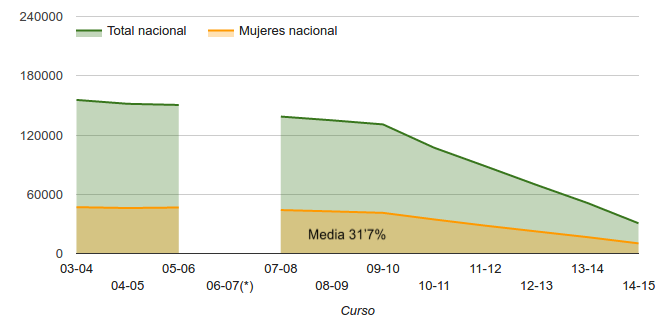
\includegraphics[width=0.75\textwidth,keepaspectratio]{Bitmap/ing_total.png}
                \label{fig:ing_total}
        }
        \subfigure[\scriptsize{Grados de Ingenierías o Enseñanzas Técnicas.}]{
                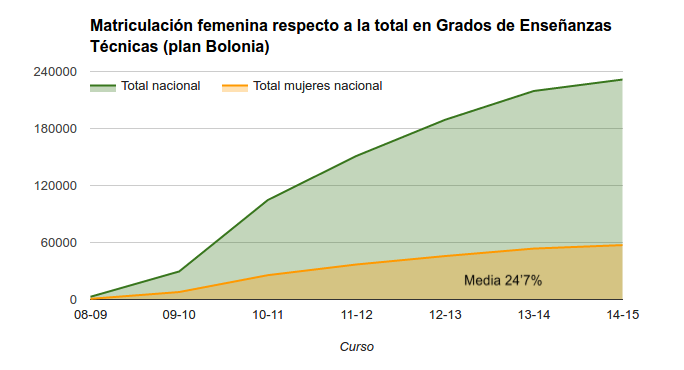
\includegraphics[width=0.75\textwidth,keepaspectratio]{Bitmap/grado_total.png}
                \label{fig:grado_total}
        }
        \caption{{\footnotesize Evolución de la matriculación de mujeres en Enseñanzas Técnicas en Universidades tanto públicas como privadas. Fuente de datos: \cite{datos::uni}.}}\label{fig:datos_total}
\end{figure}

El propósito de este artículo es el de clarificar si los factores encontrados en la literatura son válidos para un instituto de la provincia de Granada, en el cual se ha realizado un estudio mediante encuestas a estudiantes de 3º y 4º de E.S.O.\footnote{Educación Secundaria Obligatoria}, 1º y 2º de Bachillerato, y Ciclos Formativos. Para ello, en primer lugar se identificarán en la sección \ref{sec:factores} los factores que diversos estudios encontrados en la literatura han identificado como determinantes para la elección de ingenierías. Después, en la Sección \ref{sec:EdA} se estudiará el Estado del Arte según las propuestas existentes para tratar de equilibrar las cifras en cuanto cantidad de mujeres matriculadas en Enseñanzas Técnicas. La Sección \ref{sec:metodologia} detalla el contexto en el que se han hecho las encuestas, además de las razones por las que se han escogido cada una de las preguntas, así como las fuentes. Por último, en la Sección \ref{sec:resultados} se analizan los resultados obtenidos, según los tres bloques de Secundaria, Bachillerato y Ciclos Formativos, para en la Sección \ref{sec:conclusiones} ofrecer las conclusiones sobre este estudio y unas nociones sobre el trabajo futuro.

\section{Factores de influencia identificados en la literatura}
\label{sec:factores}

A la hora de identificar los factores que tienen influencia sobre los adolescentes para escoger carreras de ingeniería, no sólo nos interesa estudiar la literatura por los factores que influyen en general, sino también en función del sexo. De un estudio realizado en la Comunidad Autónoma de Cataluña \cite{everis2012}, realizado a alumnos de 3º y 4º de E.S.O. y de Bachillerato, se pueden extraer varias conclusiones. A modo general, es decir, sin tener en cuenta el sexo del alumno que responde a las encuestas, se han encontrado con que:

\begin{itemize}
  \item Los estudiantes que van mejor en asignaturas relacionadas con la tecnología, como Matemáticas, Física, Tecnología e Informática, tienden a continuar la rama tecnológica y tienen más probabilidad de querer estudiar una ingeniería. Por contra, los que van peor suelen escoger otras ramas u otras carreras universitarias.
  \item Por lo general, menos del 33\% de los alumnos de la rama de ciencias tienen claro que quieren estudiar una ingeniería.
  \item Tanto en la E.S.O. como en Bachillerato, los alumnos escogen o no una ingeniería en función de si se ven capaces para estudiarla. Este hecho se acentúa en las chicas, quienes en general se infravaloran más y tienden a creer que más que porque sea difícil, es porque ellas no se sienten capaces.
  \item El interés por las nuevas tecnologías no es determinante en la elección de ingenierías por parte de los alumnos y alumnas. También, aunque en menos medida que la capacidad, influyen de manera directamente proporcional la percepción, positiva o negativa, que tienen sobre las salidas profesionales que tienen o el prestigio que tienen los ingenieros.
\end{itemize}

Dentro de los resultados cabe destacar que, aunque no se observen estereotipos del tipo ``friki'', sí que es notable la visión sexista que se tiene de estas carreras. Así, hasta un 60\% de los encuestados totales ve las ingenierías como ``para hombres'', mientras que solo un 42\% las considera también ``para mujeres''. De hecho, cuando se les pregunta directamente por su sexo, en el informe se distingue entre E.S.O. y Bachillerato aunque los resultados muy similares. En la E.S.O., dentro del 33\% total que dice que va a estudiar un Bachillerato de ciencias, hay una diferencia del 14\% entre chicas y chicos al escoger estudios relacionados con las carreras tecnológicas. El nivel sociocultural acentúa aún más esta situación, observándose en el estudio hasta un 31\% de diferencia entre chicos de nivel socioeconómico alto y chicas de nivel socioeconómico bajo en la elección de estudios relacionados con las carreras tecnológicas. En el caso de Bachillerato, el 27\% de los encuestados asegura que va a continuar estudiando una ingeniería, aumentándose la diferencia entre chicas y chicos a un 31\%.

A la luz de estos resultados, es de interés estudiar más a fondo los factores que influencian, en particular, al colectivo femenino en la decisión de estudiar ingenierías. Para ello, se analiza el informe aportado en el proyecto ``Mind the Gap'', que será descrito de manera más extensa en el Capítulo \ref{sec:EdA}. En este informe \cite{mtg2015} se comparan tres informes previos sobre la situación de la mujer en la tecnología y en las carreras de ingeniería en los países de Holanda, Reino Unido y España.

Hay varios puntos en común entre los tres países, entre ellos que el entorno de las chicas es uno de los factores más influyentes, sobre todo la familia. Referido a este factor, no es solamente la opinión de la familia de las chicas la que influye a la hora de que escojan una carrera, sino el hecho de la concepción de la familia, observándose entre las entrevistadas que la percepción de un trabajo de muchas horas concilia poco ``con sus tareas familiares''.

Otro factor en común entre los tres países es la poca confianza que las chicas tienen en sí mismas en cuanto a enseñanzas técnicas se refiere, que encima se ve minada por la alta presencia de hombres en carreras STEM, no ayudando a que este entorno sea cómodo para ellas. Los profesores representan otro factor importante, ya que no saben cómo actuar ante la situación que se describe a pesar de que admiten que existe. Sin embargo, las autoras han observado predisposición por parte de éstos a recibir formación y nuevas metodologías para afrontar el problema en las aulas. Para finalizar los factores en común, cabe destacar que en los tres países se está de acuerdo con la necesidad de emprender acciones y organizar actividades específicas para promover las STEM entre las chicas.

Los resultados del informe del proyecto ``Mind the Gap'', que es el que se ha detallado aquí por ser el más reciente, se repiten en la mayoría de los encontrados en la literatura. Por citar algunos, en \cite{hill2010so} la AAUW\footnote{Asociación Americana de Mujeres Universitarias, o en inglés \textit{American Association of University Women}} investigó las razones de por qué hay tan pocas mujeres en las carreras o profesiones STEM, llegando a la conclusión de que las principales razones serían: la antigua creencia de que los chicos son mejores en matemáticas que las chicas, cuando este hecho se ha probado erróneo en la actualidad; el supuesto poco interés de las chicas por las STEM; y en el ámbito de empresas STEM, la conciliación familiar. 

Por último, mencionar un estudio de 2013 \cite{hazari2013factors} del que además se han incluído algunas preguntas en las encuestas realizadas y descritas en el Capítulo \ref{sec:metodologia}. En este estudio los autores pretenden demostrar cómo afectan realmente distintos factores, siendo el único influyente el discutir la poca representación femenina en la ciencia en clase.

\section{Estado del Arte}
\label{sec:EdA}

\section{Metodología}
\label{sec:metodologia}

\section{Resultados}
\label{sec:resultados}

\section{Conclusiones}
\label{sec:conclusiones}

...


\section*{Agradecimientos} 

...


%
%Hidden for double-blind review


\bibliographystyle{splncs03}
\bibliography{eleccion_grado}


\end{document}
